\documentclass[12pt, twoside, english]{report}
\usepackage{babel}
\usepackage{csquotes}
\usepackage{helvet}
\usepackage{lmodern}
\usepackage{graphicx}
\usepackage{fancyhdr}
\usepackage{geometry}
\usepackage{abstract}
\usepackage{titlesec}
\usepackage{enumitem}
\usepackage{multirow}
\usepackage{amsmath}
\usepackage{blindtext}
\usepackage{hyperref}
\usepackage{subfig}
\usepackage{pdfpages}

\usepackage{listings}
\usepackage{color}
\usepackage[dvipsnames]{xcolor}
%\lstloadlanguages{C,C++,csh,Java}

\definecolor{red}{rgb}{0.6,0,0} 
\definecolor{blue}{rgb}{0,0,0.6}
\definecolor{green}{rgb}{0,0.6,0}
\definecolor{cyan}{rgb}{0.0,0.6,0.6}
\definecolor{backcolour}{rgb}{0.95,0.95,0.96}

\lstset%
{%
    emph=[1]%
    {%
        Dictionary, string, var, function,
        async, signInWithEmailAndPassword, localStorage, querySnapshot, query, width, padding, margin, margin-bottom, border, background-color, border, box, outline,  margin-left, margin-top, webRequest, Stream, Encoding, Console, StreamReader, WebRequest, HttpWebRequest, SignInContainer, IconWrap, Icon, SignInContent, SignInForm, FormH1, LoginForm, FormGroup, FormLabel, FormInput, FormButton, Text, ImgWrapper, background-color, shadow, bottom, left, top, -, background, color, req, db, collection, stringify, await, res, doc, set, JsonConvert, JsonSerializerSettings, ReferenceLoopHandling, NullValueHandling, NodeJSON, JSONAttribute, IEnumerable, Children, Parent, TryGetValue
    },
    emphstyle=[1]{\color{cyan}},
}

\lstset{
language=csh,
basicstyle=\footnotesize\ttfamily,
numbers=left,
numberstyle=\tiny,
numbersep=5pt,
tabsize=2,
extendedchars=true,
breaklines=true,
stringstyle=\color{green}\ttfamily,
showspaces=false,
showtabs=false,
xleftmargin=17pt,
framexleftmargin=17pt,
framexrightmargin=5pt,
framexbottommargin=4pt,
commentstyle=\color{green},
morecomment=[l]{//}, %use comment-line-style!
morecomment=[s]{/*}{*/}, %for multiline comments
showstringspaces=false,
keywordstyle=\color{blue},
identifierstyle=\color{black},
backgroundcolor=\color{white}
}

\definecolor{lightgray}{rgb}{.9,.9,.9}
\definecolor{darkgray}{rgb}{.4,.4,.4}
\definecolor{purple}{rgb}{0.65, 0.12, 0.82}

\lstdefinelanguage{JavaScript}{
  keywords={typeof, new, true, false, catch, function, return, null, catch, switch, var, if, in, while, do, else, case, break, async, signInWithEmailAndPassword, localStorage },
  keywordstyle=\color{blue}\bfseries,
  ndkeywords={class, export, boolean, throw, implements, import, this},
  ndkeywordstyle=\color{darkgray}\bfseries,
  identifierstyle=\color{black},
  sensitive=false,
  comment=[l]{//},
  morecomment=[s]{/*}{*/},
  commentstyle=\color{purple}\ttfamily,
  stringstyle=\color{red}\ttfamily,
  morestring=[b]',
  morestring=[b]"
}

\usepackage[style=ieee]{biblatex}

\addbibresource{bibliography.bib}

\newcommand{\university}{Universitatea Politehnica Timișoara}
\newcommand{\studyProgram}{Calculatoare și Tehnologia Informației (limba engleză)}
\newcommand{\academicYear}{2024}
\newcommand{\firstName}{Mario-Mihai}
\newcommand{\lastName}{Mateaș}
\newcommand{\thesisTitle}{Pie - A General-Purpose Code Editor Focused on Simplicity}
% Asist.(SL/Lect./Conf./Prof.)dr.ing.(arh./ec./chim.)
\newcommand{\coordinatorTitle}{Ș.l. dr.ing. }
\newcommand{\coordinatorFirstName}{Cosmin}
\newcommand{\coordinatorLastName}{Marșavina}
\newcommand{\candidateName}{\firstName, \lastName}
\newcommand{\coordinator}{\coordinatorTitle \coordinatorFirstName, \coordinatorLastName}
\newcommand{\CS}{C\nolinebreak\hspace{-.05em}\raisebox{.6ex}{\scriptsize\bf \#}}
\newcommand{\FS}{F\nolinebreak\hspace{-.05em}\raisebox{.6ex}{\scriptsize\bf \#}}
\renewcommand{\lstlistingname}{Code sequence}
\include{components/Format}
\include{components/Styles}

\begin{document}
\setcounter{page}{1}
\begin{titlepage}
\thispagestyle{titlepagestyle}
    \begin{center}
        \vspace*{\fill}
        \textbf{\fontsize{20pt}{30pt} \selectfont \MakeUppercase{\thesisTitle}}
    \end{center}
    
    \vspace*{\fill}
     
            
    \textbf{\fontsize{14pt}{16pt} \selectfont Candidat: \candidateName}
    
    \vspace{14pt}
    
    \textbf{\fontsize{14pt}{16pt} \selectfont Coordonator științific: \coordinator}

    \begin{center}
        \vspace{50pt}
        \fontsize{14pt}{16pt} \selectfont Sesiunea: Iunie \academicYear 
    \end{center}
    

\end{titlepage}
\newpage
\thispagestyle{pagestyle}

\begin{center}
    \textbf{\fontsize{20pt}{24pt} \selectfont Abstract}
\end{center}

Developers are in certain need of a code editor that allows them to write their programs efficiently, without having to do any additional editor configuration or manage third-party dependencies. Small-scale projects do not require the use of feature-bloated integrated development environments, which can add complexity and make the entire coding process more difficult. A good integrated development environment needs to provide the bare minimum required for decent coding, and this can be pretty difficult to achieve nowadays, as programmers rely on more and more tools to enhance the development process. The variety of technologies and frameworks doesn't help either. Developers won't rely on a single development stack when building an application, so a code editor must always be ready to support multiple languages and be constantly improved and extended.

Building a general-purpose IDE that is also easy to use and doesn't have unnecessary features is a difficult job. It requires analysis of internal and external editor tools, prioritizing their importance to such a product. I have built Pie with these aspects in mind. Pie is a general-purpose code editor that provides a consolidated suite of the most used development features, accessible from an intuitive user interface. This tool allows programmers to focus on their code, instead of constantly clicking buttons, pressing hotkeys, or skimming through the editor's documentation. The entire feature analysis has been done by me, while using Pie on a daily basis as a complete replacement for other editors.

Pie, written entirely in C\#, has been built using Microsoft's Windows Forms ("Winforms") framework and has been designed to completely replace today's popular IDEs, such as Visual Studio Code or IntelliJ, whenever their features are just too much for a certain task. The solution has also been designed as a potential replacement for smaller-scale text editors, such as Notepad++, with various integrated text editing capabilities.

The demo shown in this paper will emphasize Pie's intuitive user interface along with its main features, highlighting some of the product's use cases. A comparison between Pie and state-of-the-art text and code editors will also be performed, focusing on what my product has to offer.
\vfill
\tableofcontents

\chapter{Introduction}
\thispagestyle{pagestyle}

If we go back in time and review the history of computers, we can observe that various programming techniques have been adopted over the years. Computer programming has undergone one of the most significant evolutionary processes, beginning almost a century ago when instructions were sent to machines through plugboards and switches. Several decades later, computer engineers transitioned to punch card programming and also witnessed the release of the famous COBOL language. Some of these individuals may still be alive today, reminiscing about the times when development was not as simple as it is today.

The significant improvements from the 1930s to the present day were influenced by two major factors:

\begin{enumerate}
  \item the emergence of higher-level languages (e.g. C, FORTRAN) and languages that were built for specific purposes (e.g. Java, that redefined the way object-oriented programs were written);
  \item the constant release of tools that aided the programmer and simplified the entire development process (so-called "integrated development environments") \cite{ide_bigbang}.
\end{enumerate}

Due to the increased difficulty of maintaining (or migrating) legacy code, such as banking applications still relying on COBOL, modern tools have been developed to aid programmers even under such conditions. This means that if refactoring (or a "hotfix") is required, programmers won't need to manipulate punch cards but can simply use their keyboard and mouse, as they are already accustomed to. This situation confirms that, in several cases, integrated development environments play a more significant role than the actual programming language in the software development process. If we consider popular IDEs such as Microsoft's Visual Studio Code \cite{vscode}, we can also confirm that users are indeed able to write code even in a language they aren't familiar with, thanks to the integration of artificial intelligence.

Integrated development environments should provide every functionality needed by a software developer while working on a project. However, there are several cases where such a tool provides more than required, and using it may become a burden for the user \cite{ide_productivity}. IDEs were built to make the entire coding process more time-efficient, but they do exactly the opposite when the developer isn't accustomed to their features or when using such a tool for a small-scaled application. In the same manner, moving on to a "simpler" editor, such as Notepad++, which focuses primarily on text editing, might also not be a good solution, as it may not provide all the necessary tools for development.

With this in mind, I have implemented Pie: a lightweight code editor, useful for scripting or coding small projects that do not require the feature bloat available in today's popular IDEs. Pie provides text editing capabilities, similar to Notepad++, but it also integrates features most commonly required during application development. These capabilities include: code syntax highlighting and autocomplete, text formatting options, visualization of data available via the persistence layer, local repository management, and the ability to store and access custom build commands. Additionally, Pie provides real-time rendering of HyperText Markup Language (HTML) and Markdown code. All of these features can be accessed through a docked menu strip, where they are classified into categories and subcategories. Apart from the top menu, Pie's interface displays only the developer's main focus area - either the code editor, the output of a rendered HTML page, or the current status of the local git repository - with no other controls that might distract the user displayed unless explicitly toggled. 

As previously mentioned, the project is a general-purpose code editor, providing support for the most commonly used programming languages today. These include, but are not limited to: C, C\#, Java, JavaScript, JSON, Lua, Python, XML, HTML, and SQL. Pie has also been intended to be fully customizable. In addition to saving commands and storing database connection information, users can completely alter its color combinations. I have included several default themes that I believe look appealing; however, users are free to modify these or extend the list by adding their own custom themes.

Pie is a free software solution, designed as an open-source product from its first day of implementation. It is the result of more than a year of intense work and refinement, although it was not initially intended for use as a diploma project. I aimed to create a product that would assist me in situations where an IDE was just too much. Throughout the implementation process, I used Pie as my primary code and text editor, completely replacing Notepad and Notepad++. Whenever I realized that I needed a quicker way to perform a task, such as removing duplicate lines in text, and anticipated using this feature more than once, I would close everything and begin developing that feature.

The rest of the paper will be structured as follows: Chapter 4 presents similar products that were used as sources of inspiration for Pie, detailing differences and similarities between my product and state-of-the-art IDEs. Architectural aspects are considered in Chapter 5, along with the frameworks and third-party dependencies I have used. This chapter will also present the structure of the application, emphasizing the five main components that make up Pie. The implementation of Pie is discussed in Chapter 6, where I will present several code snippets that show how the user interface logic is separated from the business logic of the application. A demonstration of the project will be displayed in Chapter 7, while we conclude the paper and mention future work in Chapter 8.
\chapter{Actual state of the art}
\thispagestyle{pagestyle}

\section{Evolution of code editors over an entire century}
\subsection{Punch card programming}

Long before the appearance of floppy disks, magnetic tape and hard drives, programmers had an entire different way of communicating with machines. In the late 1920's, not even the first procedural languages were introduced, and the most efficient way of sending instructions to a computer back then was through so-called "punch cards".

Punch cards were designed to hold data. Such data would be stored by punching holes, which represented either letters or numbers. A character was being represented through a hole in a column. An entire line of code could be written by punching holes in about 80 bytes of rows and columns, which took an entire punch card \cite{ibm}.

Improved versions of the punch card were introduced during the following decades, but the process remained very similar, and improvements weren't as observable as they are today. Programming was still a process that required a clear and sharp mind, and couldn't be done as easily as in the present. Syntax errors in the punch card era often required the program to be rewritten from the start, as those holes couldn't be filled back.

\begin{figure}[h]
\centering
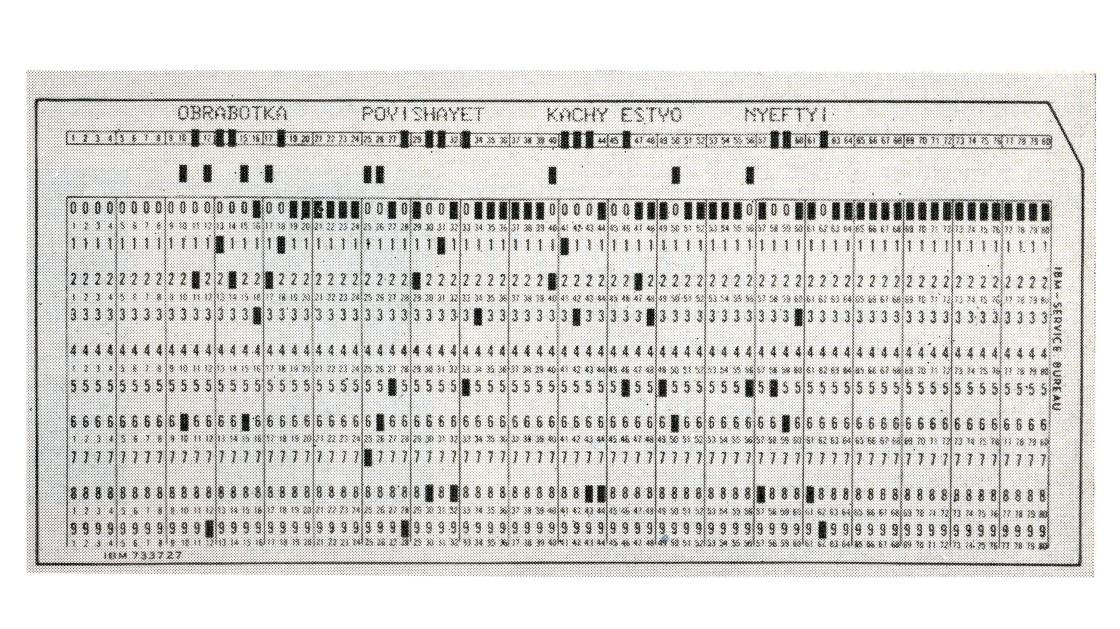
\includegraphics[width=0.5\textwidth]{images/punchcard.jpeg}
\caption{An 80-column Russian-translation punched card from 1954}
\label{fig:fig2,1.}
\end{figure}

Later, the punch card creation process was simplified thanks to the appearance of keypunch machines, which allowed code to be written using an early version of the keyboard. The machine automatically punched holes in the cards, eliminating the need for the programmer to do it manually.

\begin{figure}[h]
\centering
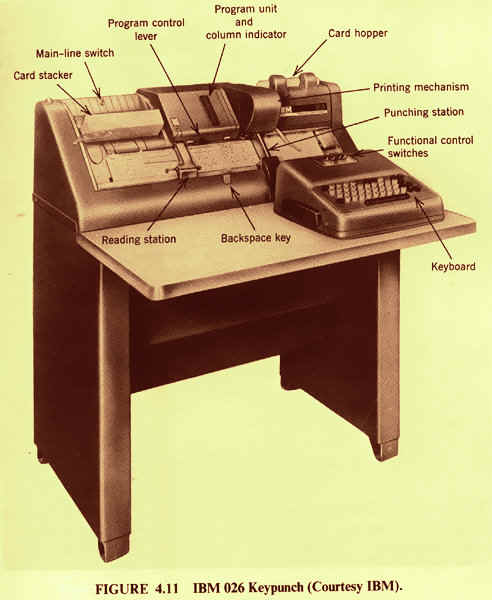
\includegraphics[width=0.5\textwidth]{images/keypunch.jpg}
\caption{The IBM 026 Key Punch}
\label{fig:fig2,1.}
\end{figure}

\subsection{First digital text editors}

A significant leap from punch cards was represented by the so-called TECO (Text Editor and Corrector), a text editor originally developed on the PDP-1 by Dan Murphy. Its release took place in 1962, more than six decades ago, and TECO is still included in some operating systems such as OpenVMS.

Even though TECO did not provide syntax highlighting and autocomplete features, it redefined the standards of text editing software by offering unique capabilities for searching and modifying text through its "macros".

In 1979, a new editor called vi entered the market. Vi was designed as a modified version of two editors written for UNIX systems: the popular ed ("editor"), which was natively integrated into UNIX, and em ("editor for mortals"). Em was a modified version of ed, created by George Coulouris.

Vi was developed by Bill Joy, a student at the time, who was dissatisfied with the capabilities of state-of-the-art editors while fixing a Pascal compiler \cite{vi}. Its ease of use and simplified user interface provided a significant advancement over TECO, which, though very powerful at the time, was considered too advanced for those who didn't want to learn all of its commands.

The introduction of mnemonic commands to manipulate text brought editors one step closer to the intuitive user interfaces we see today in modern software. However, the original vi still didn't include syntax highlighting features. A modified version of vi, called vim ("vi improved"), was released a decade later. Both editors have been included in UNIX's toolset.

\begin{figure}[h]
\centering
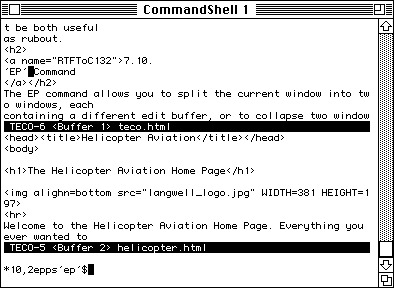
\includegraphics[width=0.5\textwidth]{images/teco.jpg}
\caption{Text Editor and Corrector (also known as TECO)}
\label{fig:fig2,1.}
\end{figure}

\begin{figure}[h]
\centering
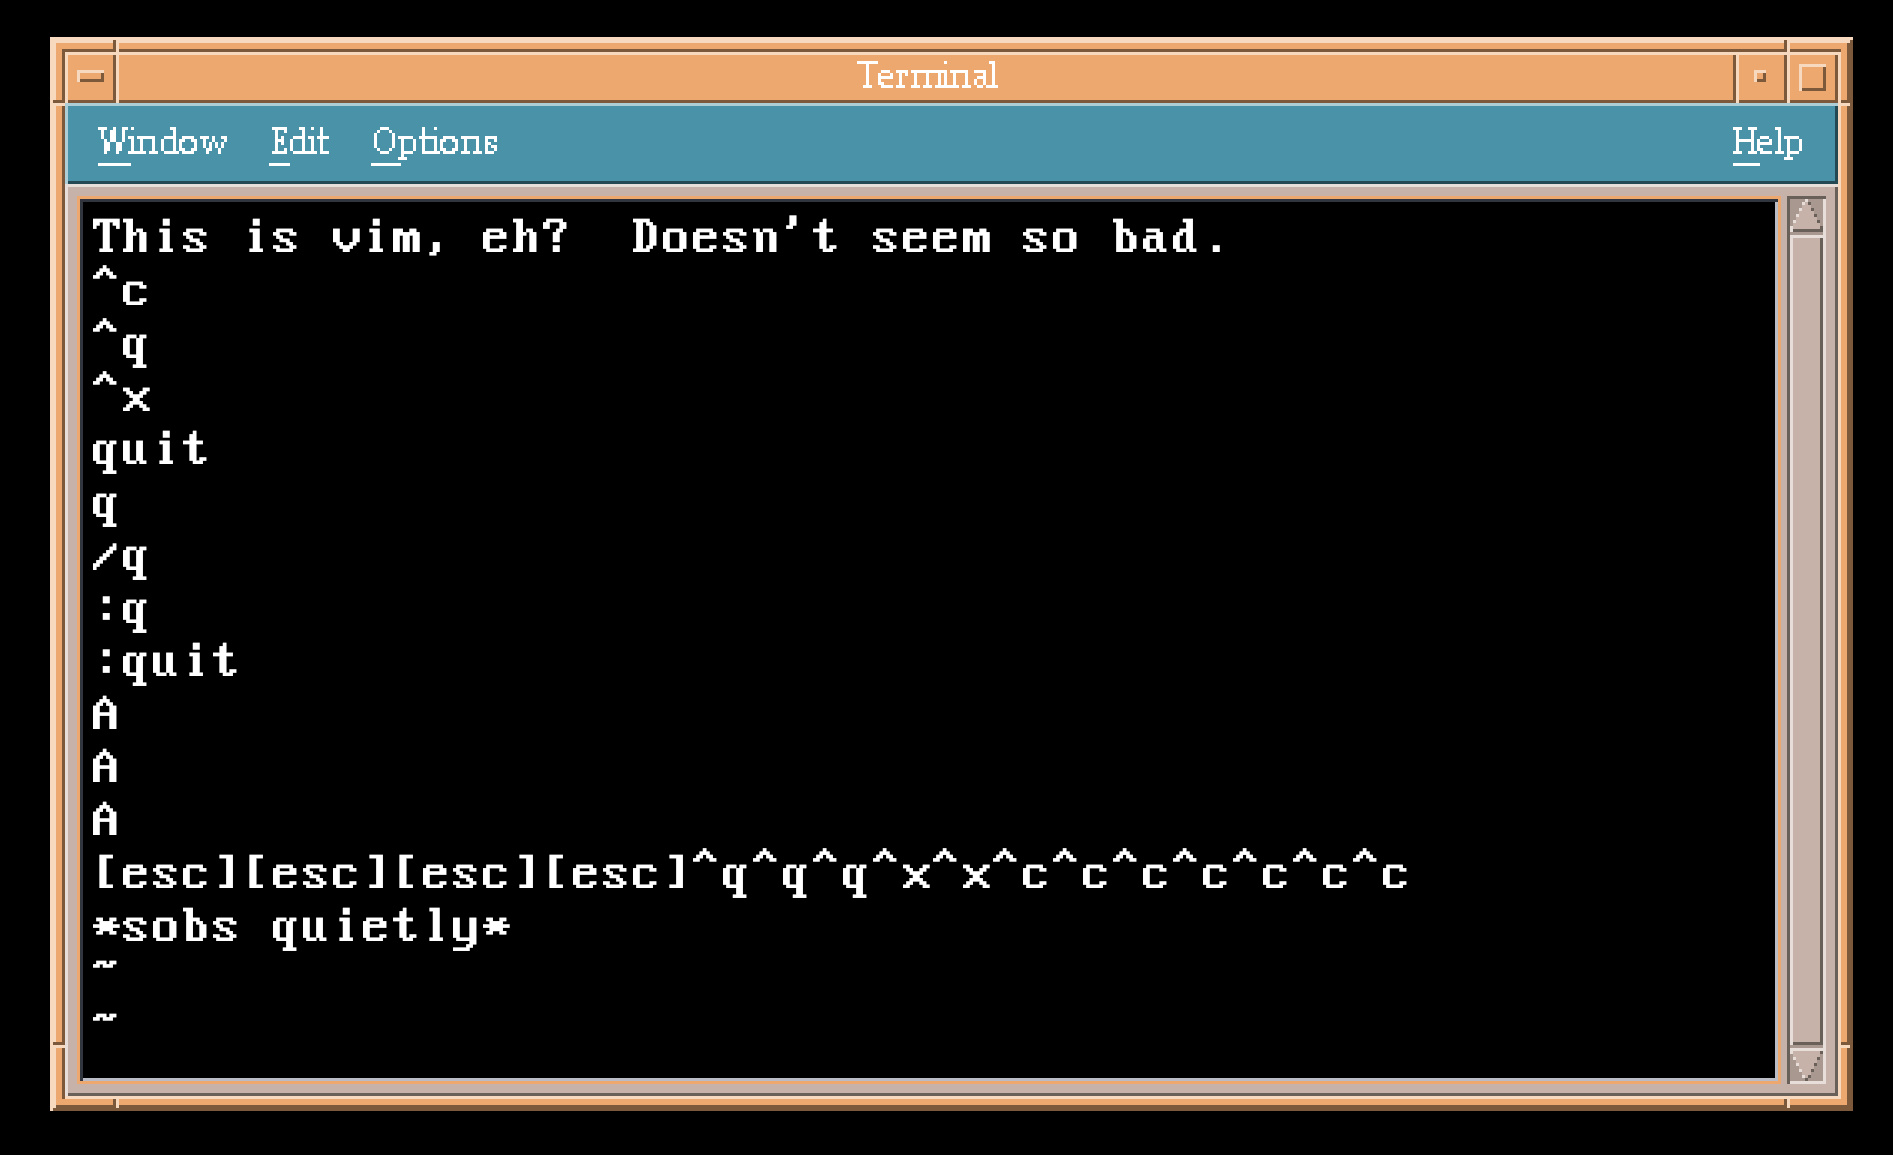
\includegraphics[width=0.5\textwidth]{images/vi.png}
\caption{vi editor}
\label{fig:fig2,1.}
\end{figure}

\subsection{Integrated Development Environments}

Several years after the release of vim, in 1991, developers realized that software projects were becoming larger and more complex than ever before. Microsoft released its first version of Visual Studio in 1997, and Eclipse launched its first open-source IDE, primarily oriented towards Java development.

Software products began to rely more on graphical user interfaces (UI), requiring intensive use of third-party dependencies and frameworks. Build tools such as Apache Ant and Maven were introduced to simplify the building process of hundreds or even thousands of files.

Terminals and command-line tools could no longer be considered acceptable media for building projects. With the release of popular frameworks such as .NET (2002), Spring (2002), and Django (2005), integrated development environments (IDEs) became the best option for software developers.

IDEs came with many features that aided the entire coding process. Refactoring, the ability to change a field's name in a class definition while automatically updating references in all of the project's files, was revolutionary at the time. Debuggers, build automation, code coverage tools, and source control management were all considered innovative and extremely helpful. Developers no longer needed to rely on external tools, as IDEs had everything packed into a single software product.

\begin{figure}[h]
\centering
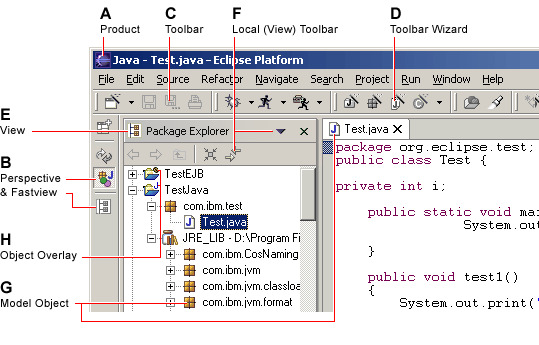
\includegraphics[width=0.5\textwidth]{images/eclipse.jpg}
\caption{Eclipse User Interface (2004)}
\label{fig:fig2,1.}
\end{figure}

\begin{figure}[h]
\centering
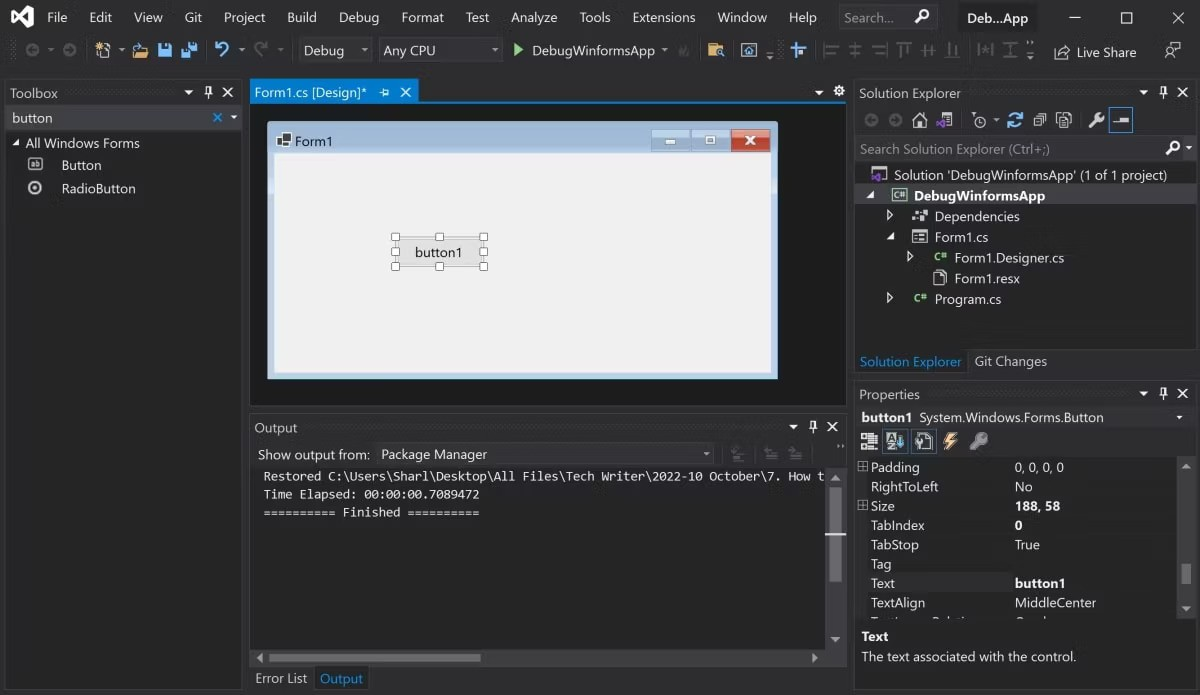
\includegraphics[width=0.5\textwidth]{images/visual_studio.jpg}
\caption{An actual version of Microsoft Visual Studio, featuring Drag and Drop capabilities}
\label{fig:fig2,1.}
\end{figure}

\subsection{Rise of modern code editors}

After years of continuous improvements in IDEs, it became clear that smaller projects also required a suitable medium for development. Python, although released in 1991, gained significant popularity almost 20 years later. Besides being used in frameworks such as Django and Flask, Python was also intended for scripting. Eclipse, NetBeans, and Visual Studio were not designed for projects with a smaller number of source files. While integrated development environments improved time efficiency for enterprise projects, they had the opposite effect for Python scripts or static web pages.

Text editors had already seen modern implementations, such as the release of Notepad++ in 2003, but the product was mainly intended for text formatting and manipulation, despite providing several code editing features.

Code editors, which primarily focused on assisting developers in the process of writing code rather than on the project's build process, began to be released. This started with Sublime Text (2008), and continued with the popular Visual Studio Code (2015), a lightweight, general-purpose adaptation of Visual Studio.

Nowadays, code editors are statistically the preferred option for frontend development, scripting, and small programs that can be compiled using the command line.

\begin{figure}[h]
\centering
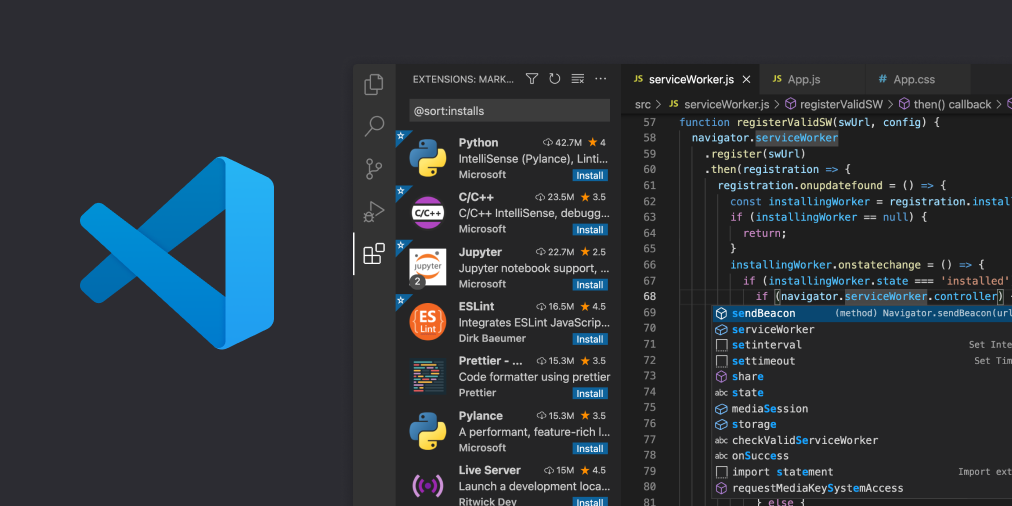
\includegraphics[width=0.7\textwidth]{images/vscode.png}
\caption{Microsoft Visual Studio Code's user interface}
\label{fig:fig2,1.}
\end{figure}

\section{Pie - An Editor Focused on Simplicity}

\subsection{The reason Pie was developed}

Smaller projects are not meant to be developed using heavyweight tools. The release of Visual Studio Code has significantly improved the process of creating small-scale applications. However, during the years, code editors such as the one mentioned before faced changes and feature additions that increased the complexity of use.

Visual Studio Code, although marketed as a tool easy to use ("Edit, build, and debug with ease" \cite{why_vscode}), bases almost its entire configuration on JSON-formatted files. Adding custom build commands (called "Tasks") requires manual editing of a tasks.json file.

\begin{lstlisting}[language=json, caption={tasks.json configuration for compiling C sources in Visual Studio Code}]
{
  "version": "2.0.0",
  "tasks": [
    {
      "label": "build",
      "command": "gcc",
      "args": ["-Wall", "helloWorld.c", "-o", "helloWorld"],
      "problemMatcher": {
        "owner": "cpp",
        "fileLocation": ["relative", "${workspaceFolder}"],
        "pattern": {
          "regexp": "^(.*):(\\d+):(\\d+):\\s+(warning|error):\\s+(.*)$",
          "file": 1,
          "line": 2,
          "column": 3,
          "severity": 4,
          "message": 5
        }
      }
    }
  ]
}
\end{lstlisting}

This code snippet is extracted from \href{https://code.visualstudio.com/docs/editor/tasks}{https://code.visualstudio.com/docs/editor/tasks}.

\hspace{0pt}

Besides from that, its language support capabilities are entirely based on extensions that need to be downloaded from an integrated download manager called "Extension Marketplace".

\begin{figure}[H]
\centering
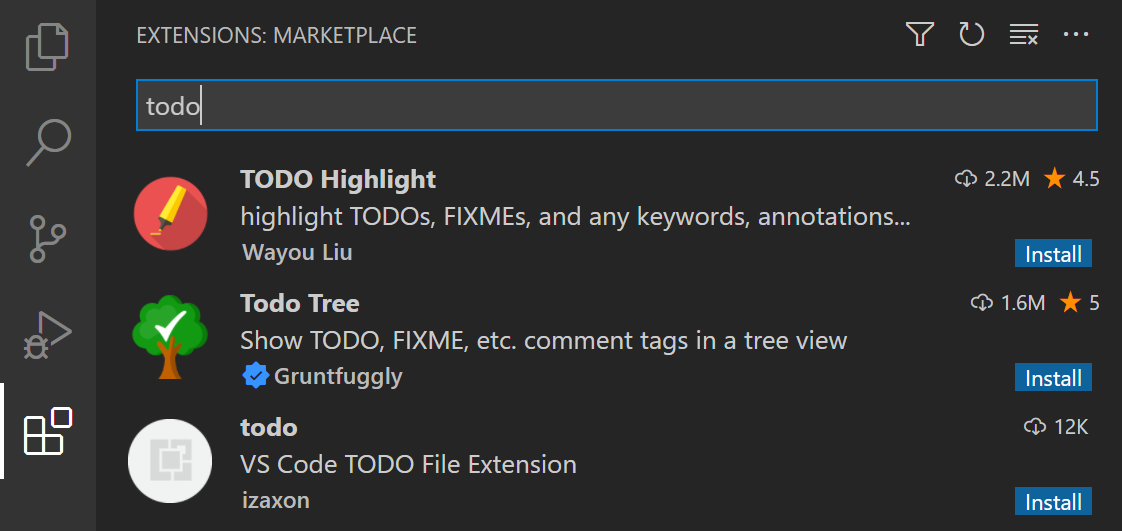
\includegraphics[width=0.5\textwidth]{images/vscode_extensions.png}
\caption{Microsoft Visual Studio Code's "Extension Marketplace"}
\label{fig:fig2,1.}
\end{figure}

Additional settings are also very difficult to find, due to Visual Studio Code's complex user interface. Popup windows and unnecessary sidebars keep the programmer away from their main focus area - the actual code editor.

Although Visual Studio Code may seem like a good option for more complex web applications or scripts, using it on a daily basis for editing small text or source files is not what it was intended for.

Moving further to the option that may seem the best for the use cases described above, Notepad++ seems to be the editor that is capable of doing everything. It provides code support, text manipulation capabilities, and its interface is also configurable. However, many people still decide not to rely on it for their daily tasks.

Notepad++ has been released in 2003 and it hasn't updated its interface very much since then. It is oriented more towards text manipulation, as it lacks commonly used development features such as integrated terminal and version control management system. Advanced features can, indeed, be added to Notepad++, but the product requires installation of additional plugins, similar to Visual Studio Code's "extensions" system.

\begin{figure}[H]
\centering
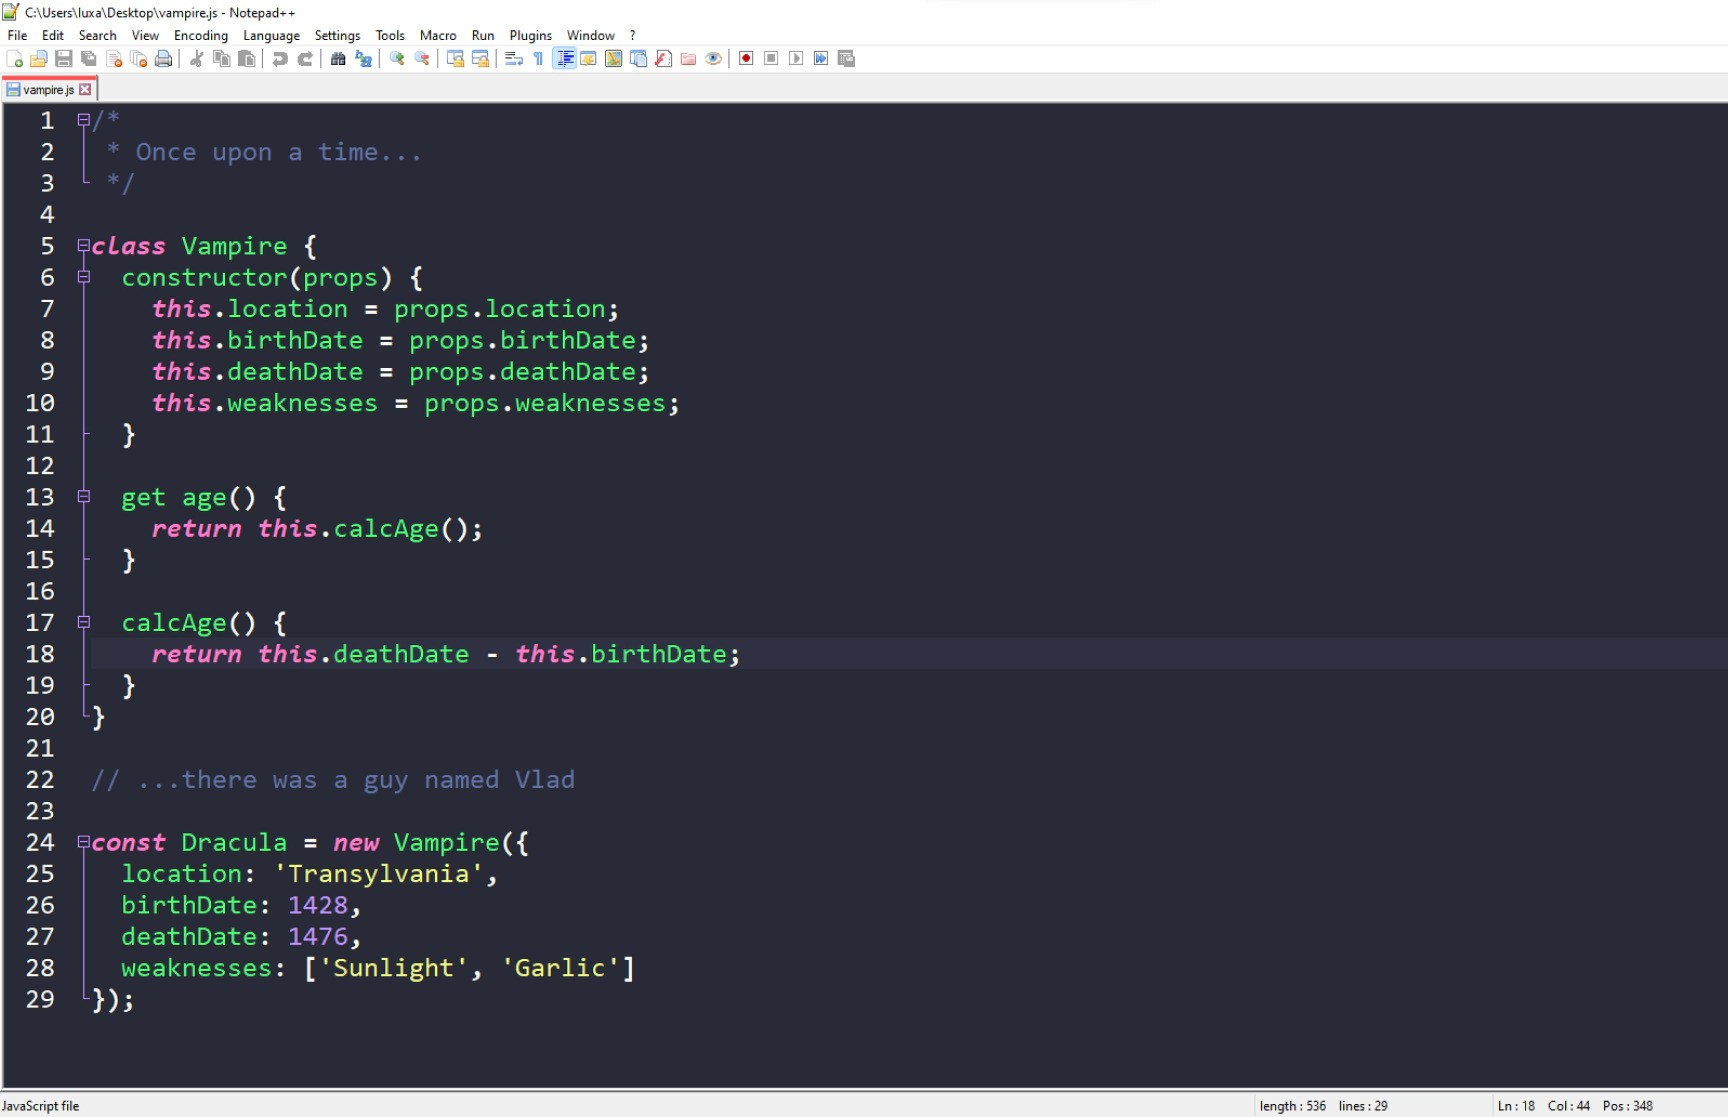
\includegraphics[width=0.8\textwidth]{images/notepad-plus-plus-dark.jpg}
\caption{Third-party "Dracula" theme for Notepad++, only changes the color of the text editor, leaving design inconsistencies}
\label{fig:fig2,1.}
\end{figure}

I have designed Pie with the purpose to fill in the lacks of Notepad++, while also keeping its user interface simple and accessible to every user. An editor made for daily use should be fast, simple and robust.

\subsection{Comparing Pie with state-of-the-art editors}

Similar to popular code editors, Pie offers syntax highlighting and code autocomplete features for various programming languages. These features are automatically toggled based on the extension of the opened file. Syntax highlighting is considered an essential feature of integrated development environments, as it has a massive impact on code comprehension \cite{syntax}.

The aspect that makes the biggest difference between Pie and potential competitors is the user interface. Pie has a user interface as clean as the classic Notepad while still offering most of what is needed for a proper development session. Compared to Notepad++ or Visual Studio Code, all of Pie's features are properly organized into categories and subcategories, making them accessible in seconds.

\begin{figure}[h]
\centering
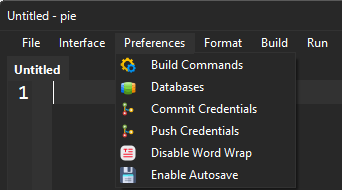
\includegraphics[width=0.5\textwidth]{images/pie-menu-strip.png}
\caption{Pie's docked menu strip, featuring the "Preferences" category}
\label{fig:fig2,1.}
\end{figure}

Pie also comes with a set of integrated development tools, such as a repository explorer for Git, a database connection manager, and integrated terminals. A vanilla version of Notepad++ doesn't provide such capabilities and requires installation and configuration of third-party plugins, which may present unexpected behavior since they are not designed by the product's original authors. Visual Studio Code offers several of these features without requiring users to navigate through their Extension Marketplace. However, because of its complex configuration model present in every aspect of the application, it requires users to spend minutes or even more to make them work as intended.

Visual Studio Code, assisted with third-party extensions, provides everything required for properly managing a database. The "Oracle Developer Tools for VS Code (SQL and PLSQL)" allows users to manipulate tables and entries the Oracle-way. However, most of these features are only required in special cases. For example, an SQL script that runs against one's database whenever a connection is established may be a good way of keeping the database secure, but it certainly isn't needed for a smaller project or for a prototype application.

\begin{figure}[h]
\centering
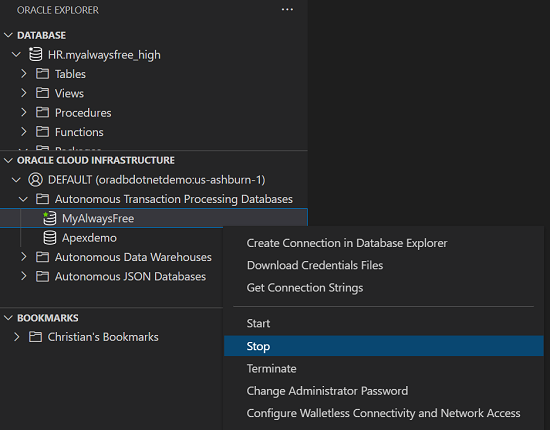
\includegraphics[width=0.6\textwidth]{images/oracledb-vscode.png}
\caption{Oracle Database connection management in Visual Studio Code}
\label{fig:fig2,1.}
\end{figure}

Pie's database connection manager is as simple as it sounds. Users add their connection details and are able to launch SQL scripts against every file with an .sql extension, directly from the context menu. No special environment needs to be opened. Whenever the user navigates through a project directory and finds an SQL file, they can directly run it against a database.

Comparing other Visual Studio Code aspects, their "Task" functionality, already mentioned in the previous subsection, allows users to input their own custom commands, which may be executed at any time. Most of the build commands are going to be executed manually by the user. Working on smaller projects won't require specifying which file patterns or directories should be built. Compared to Visual Studio Code's Tasks, Pie's "Build Commands" interface is much simpler.

\begin{figure}[H]
\centering
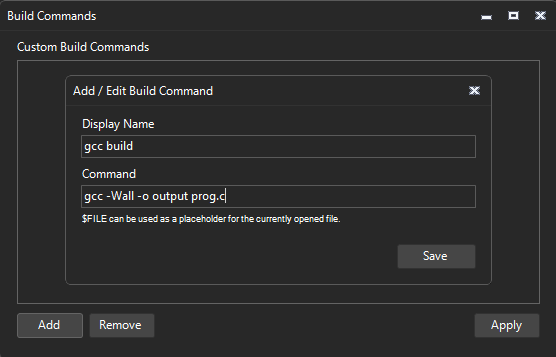
\includegraphics[width=0.6\textwidth]{images/pie-build-commands.png}
\caption{Adding a gcc build command in Pie}
\label{fig:fig2,1.}
\end{figure}

Compared to Notepad++, which is focused on text editing, Pie has several capabilities used for the same purpose. It won't be able to replace Notepad++ in special cases, where intense text manipulation is required, but its "Format" features offer most of what is required on a daily basis. Sorting a list, removing duplicate lines or lines consisting only of whitespaces are simplified ways of cleaning input or output data. Such data will be often present in software projects, no matter the size, so it was essential for them to be integrated into Pie.

The table below depicts a comparison between most popular integrated development environments or code editors and Pie. As observed, the debugging functionality is not present into Pie, because integration of specific compilers would have been required, and my product was not designed for that purpose.

\begin{table}[h]
\centering
\scalebox{0.7}{
\begin{tabular}{|*{7}{c|}}
\hline
 & \textbf{Visual Studio Code} & \textbf{Sublime Text} & \textbf{Notepad++} & \textbf{IntelliJ IDEA} & \textbf{Atom} & \textbf{Pie} \\
\hline
\textbf{Syntax Highlighting} & \checkmark & \checkmark & \checkmark & \checkmark & \checkmark & \checkmark  \\
\hline
\textbf{Autocomplete} & \checkmark & \checkmark & \checkmark & \checkmark & \checkmark & \checkmark  \\
\hline
\textbf{Automatic Indentation} & \checkmark & \checkmark & \checkmark & \checkmark & \checkmark & \checkmark  \\
\hline
\textbf{Code Folding} & \checkmark & \checkmark & \checkmark & \checkmark & \checkmark & \checkmark  \\
\hline
\textbf{Advanced Text Manipulation} & P & $ \times $ & \checkmark & P & P & \checkmark  \\
\hline
\textbf{Integrated Terminal} & \checkmark & P & P & \checkmark & P & \checkmark  \\
\hline
\textbf{Debugger} & \checkmark & P & $ \times $ & \checkmark & P & $ \times $  \\
\hline
\textbf{Custom Build Commands} & \checkmark & \checkmark & \checkmark & \checkmark & \checkmark & \checkmark  \\
\hline
\textbf{Git Integration with UI} & \checkmark & $ \times $ & $ \times $ & \checkmark & \checkmark & \checkmark  \\
\hline
\textbf{Integrated HTML Preview} & P & $ \times $ & P & \checkmark & P & \checkmark  \\
\hline
\textbf{Integrated Markdown Preview} & P & $ \times $ & P & \checkmark & P & \checkmark  \\
\hline
\textbf{Execute SQL queries} & P & P & $ \times $ & \checkmark & P & \checkmark  \\
\hline
\textbf{Customize application colors} & \checkmark & \checkmark & $ \times $ & \checkmark & \checkmark & \checkmark \\

\hline
\end{tabular}}
\vspace{2mm}
\caption{Feature comparison of popular integrated development environments, compared with Pie\\
(\checkmark - feature available, $ \times $ - feature not available, P - feature available only with installed plugin)}
\end{table}

We can now conclude the reasons Pie was developed, and why it is different from state-of-the-art IDEs:

\begin{enumerate}
  \item user interfaces in popular modern editors have become overly complex, making it difficult for new or casual users to locate essential features within the editor;
  \item integrated development environments do not emphasize commonly used features, they come with a large set of functionalities, most of them being used only in very specific cases;
  \item editors designed for daily tasks, like Notepad++, have been developed over decades but typically offer only the minimum required for software development, programmers being forced to switch between multiple apps or use additional external tools. 
\end{enumerate}

Pie is designed to be used for everything, from basic text editing and scripting, to software development, whenever it feels to much to use an integrated development environment.
\chapter{Technologies}
\thispagestyle{pagestyle}

Pie's technologies were chosen with maintainability in mind. I have integrated various technologies and third-party libraries already used in popular mature open-source projects. Such technologies are backed up by large communities and frequent updates, confirming that they will not become obsolete in the near future.

\section{Microsoft's Windows Forms and the .NET Framework}

THE .NET Framework was introduced in 2001 by Microsoft, together with the Visual Studio tool. It was built for the purpose to simplify Windows application development \cite{net-framework}, currently supporting three languages, also developed by Microsoft: Visual Basic, a user interface adaptation of the BASIC language, C\#, and F\#.

Pie uses Windows Forms (commonly referred to as "WinForms"), as the primary technology for its graphical user interface and business logic. WinForms is a technology that was introduced with the first version of .NET. It "can be thought of as a wrapper around the complex Win32 API" \cite{winforms-history}. The solution 
simplified desktop development by allowing programmers to focus on the business logic, instead of coding user interface components. Components, officially known as "Controls", could be added to application windows (or "Forms") simply by dragging and dropping them on the workbench.

Although not the first WYSIWYG ("What You See Is What You Get") designer, Windows Forms is certainly one of the most popular ones, as it came directly from Microsoft, the developer of Windows, receiving frequent updates and support even to this day. It is also available for all of the three .NET languages. I have chosen C\#, as it is the most commonly used among them.

WinForms is not the only user interface technology developed by Microsoft. Several years later, in 2006, Windows Presentation Foundations ("WPF") has been introduced, followed by the Universal Windows Platform ("UWP") technology in 2015. Although the latter provide a more actual way of splitting user interface logic and business logic, Windows Forms received more support during the years, is simpler to use, and has more compatible extensions ready to be integrated. Windows Forms is also considered to be a better option, from a memory management point of view. Performance is also a key to be taken into consideration, and in this manner, it seems that there is no significant difference between newer technologies such as WPF and WinForms \cite{han2023optimization}. Even so, the Form components inside Pie do not incorporate a large number of controls (e.g. buttons, textboxes, labels, panels) and the file handling logic is as simple and possible, using actual C\# integrated methods. Thus, the application is not expected to cause any slow-downs during the start-up or the usage of it.

The "Form" control is a representation of any window displayed in an application. The Form class can be used to create standard, floating and borderless windows. The "Properties" panel (present in any type of Control object), can be used to determine the appearance, size, color and window management features of the windows or dialog boxes that are created. \cite{form-class}

\begin{figure}[H]
\centering
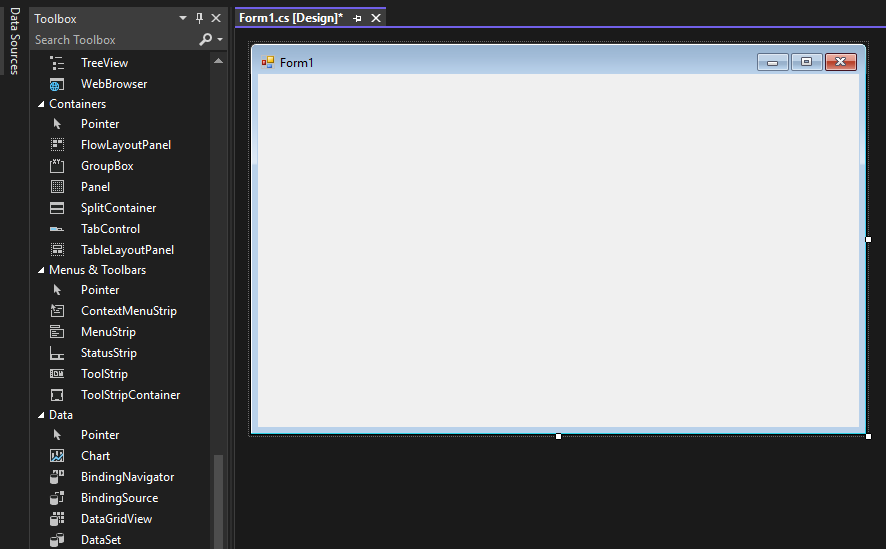
\includegraphics[width=0.8\textwidth]{images/winforms-designer.png}
\caption{Designing a Form using the WinForms technology in Visual Studio}
\label{fig:fig2,1.}
\end{figure}

Controls (available in the "Toolbox" sidebar of the designer) can have certain "Events" attached to them. Events can be triggered on several occasions:

\begin{enumerate}
  \item a mouse is hovered over the control;
  \item the control is clicked;
  \item someone presses a key, while holding focus on the control. 
\end{enumerate}

Pie uses a large number of event handlers, being able to respond to certain key bindings accordingly. Thus, users can toggle different user interface components such as the Find\&Replace dialog or the integrated terminal system simply by pressing a predefined key combination. 

The NuGet pacakge manager, integrated into Visual Studio, is the most effective and secure way to add external libraries to a .NET project. It provides a large collection of packages built by developers, including file parsers, user interface components, or database drivers, ready to be bundled into the application.

\begin{figure}[H]
\centering
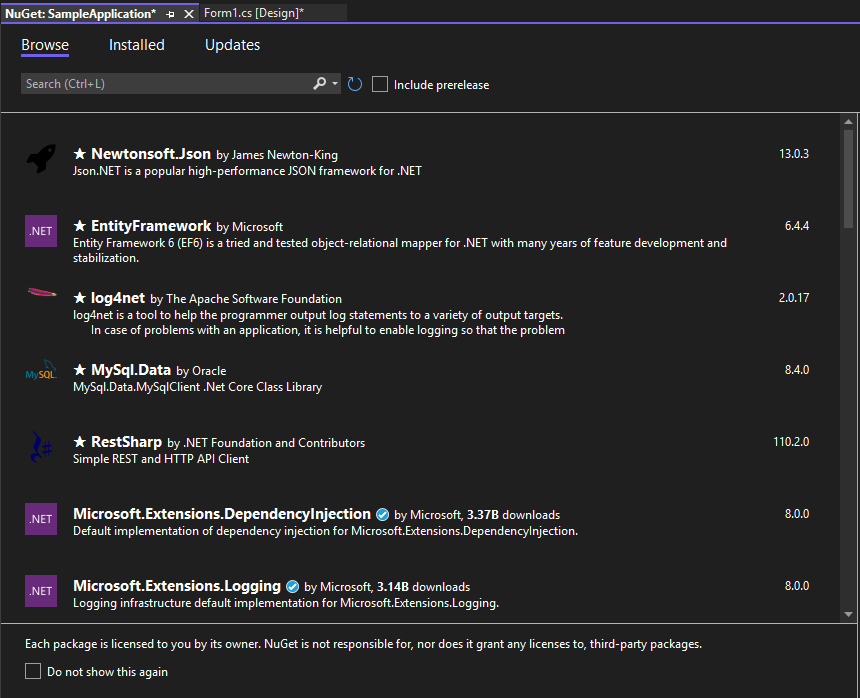
\includegraphics[width=0.8\textwidth]{images/nuget.png}
\caption{Using NuGet to discover packages available to install in a Windows Forms application}
\label{fig:fig2,1.}
\end{figure}

\section{Third-party libraries included with Pie}
\subsection{Redesigning .NET components with Krypton and ObjectListView}

Even though WinForms offers a vast toolbox of controls and customization options, it still has its limitations when it comes to design of native Windows elements. While most of the components can be customized, this typically requires writing complex event handling logic and overriding methods from the framework's base classes. In order to minimize the default Windows look in my application, I have integrated a third-party library called Krypton \cite{krypton}.

Krypton provides a better way to personalize the overall design of WinForms controls through the integration of the "KryptonPalette" class. A singleton instance of this class is accessible from all components in the application, including forms, panels, buttons, and labels. I have defined a general color scheme and other design aspects, such as border rounding and label font size, and have configured all project components to inherit their properties from this singleton.

Another limitation of Windows Forms is the ListView control. A ListView is used to display multiple elements in a list \cite{listview}, being able to handle events such as mouse clicks, mouse hovers, and key presses. However, neither the native ListBox integrated into Visual Studio nor Krypton's implementation of the ListView offers the level of customization needed for my application. To address this, I have integrated the ObjectListView \cite{objectlistview} library into the project.

ObjectListView allows for the mapping of actual objects (not just strings) to ListView controls, and offers a way to assign icons or specific colors to each element based on specific fields. This "Object-to-ListView" mapping was a requirement for Pie, as the control is used to display the status of the files in Git repositories, the list of custom build commands, and the database connections added to the application.

\subsection{Relying on Newtonsoft.Json to parse configuration files}

Pie stores configuration files such as color scheme definitions and Git credentials in JSON-formatted files. JSON is preferred over popular formats like XML, when simple data is transmitted, and the focus is on the data handling performance \cite{json-vs-xml}.

Whenever the user does a change in the configuration of the application, a JSON file needs to be rewritten. In the same manner, whenever Pie is started, the entire configuration specified in the JSON files needs to be loaded internally. A proper way of handling these files is through the Newtonsoft.Json \cite{newtonsoft-json} parsing library.

Newtonsoft.Json is used to deserialize (read) JSON files into internal configuration objects and to serialize (write) these objects back into JSON files in an efficient manner, without introducing any noticeable temporal overhead.

\subsection{Integrating the code editing functionality with Scintilla}

The most used control, the actual code editor, is an instance of ScintillaNET \cite{scintillanet}, a C\# wrapper implemented over the famous Scintilla \cite{scintilla}, also used by Notepad++ and Code::Blocks.

Scintilla is an advanced code editing component that can be customized up to anyone's preferences, providing syntax highlighting, code folding, line numbering and code breakpoints. It was developed and released by Neil Hodgson in 1999 and it is still being maintained to this day. 

ScintillaNET provides a better and easier way to integrate Scintilla inside .NET applications, being fully intended for the Windows Forms platform. This aspect can be used as a solid argument to justify my decision of using WinForms as Pie's GUI framework. Several pre-defined Scintilla lexers were already integrated inside the library (e.g. C, Python, Lua), and I have additionally included code from other open-source lexers. Syntax highlighting for languages similar to C, such as Java, use the pre-defined C lexer, but I have modified the list of keywords, based on official documentation found online \cite{java-keywords}.

\begin{figure}[H]
\centering
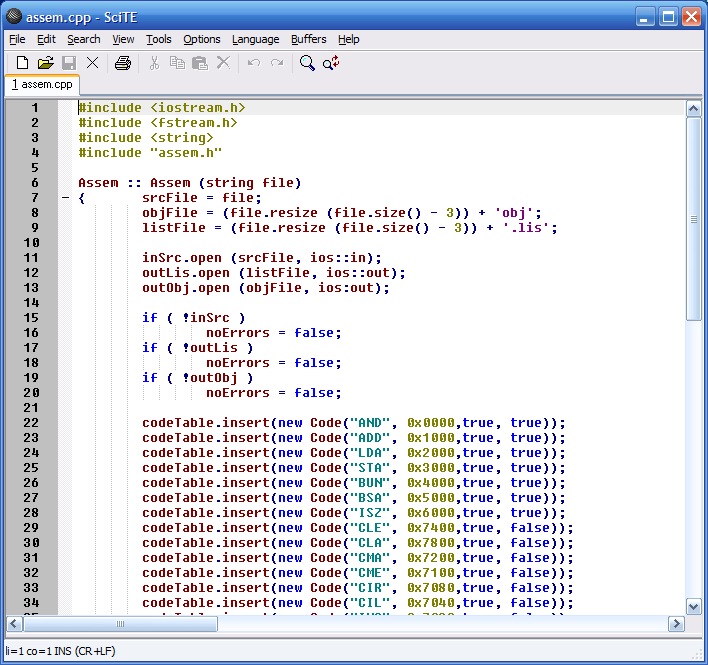
\includegraphics[width=0.7\textwidth]{images/scite.png}
\caption{Scintilla's syntax highlighting capabilities in the SciTE editor}
\label{fig:fig2,1.}
\end{figure}

Syntax highlighting may not be enough for some developers, and with this in mind, I have also integrated autocomplete functionality for the languages supported by Pie. This has been made possible through the AutoCompleteMenu-ScintillaNET \cite{autocompletemenu} library. It suggests autocomplete for the keywords of a specific language, identified by the extension of the opened file.

\subsection{Terminal instance management using ConEmu}

Pie allows users to manage an unlimited number of terminal instances during their working session. At this moment, developers are only able to automatically launch Command Prompt or PowerShell processes, but navigating through other terminals (such as bash) is possible through the command line. Output of custom builds is also redirected to an integrated terminal instance, with a new window created every time the user clicks on a saved build command.

This functionality was made possible by adding the ConEmu Inside \cite{conemu-inside} package, an extension of the popular ConEmu \cite{conemu} terminal for Windows. ConEmu is a free open-source terminal emulator launched in 2007, that was initially intended as a companion to a mature file manager for Windows. It sparked interest two decades ago with its capability to bypass several standard Windows console host features, being still used to this day.

\begin{figure}[h]
\centering
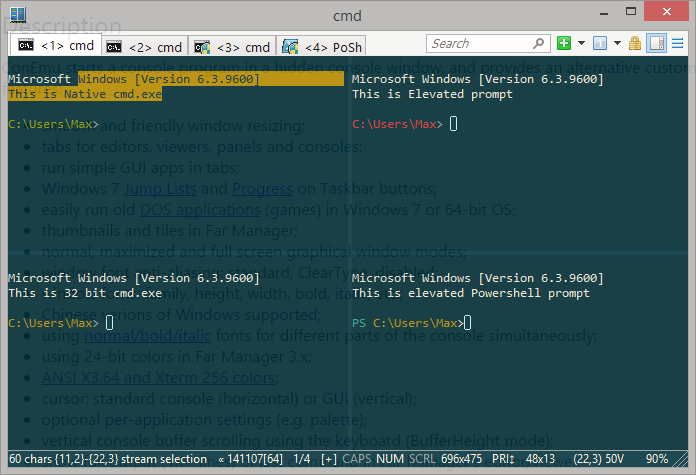
\includegraphics[width=0.8\textwidth]{images/ConEmu-Maximus5.png}
\caption{Graphical User Interface (GUI) of the ConEmu terminal}
\label{fig:fig2,1.}
\end{figure}

\subsection{Using CefSharp and Markdig for rendering code inside web browsers}

Pie provides a rendering functionality that displays HTML code in a web browser window, integrated directly inside the application. Although Microsoft's native web browser API for WinForms is able to receive HTML code and render it, it isn't updated regularly and doesn't handle JavaScript well. The engine used for .NET's WebBrowser control is based on the old Internet Explorer. For this purpose, I have used CefSharp \cite{cefsharp}, a C\# wrapper over the Chromium framework, that allows an efficient way of operating on web pages, thanks to its multithreaded implementation \cite{mohamed2022performance}.

I have also provided Markdown rendering support, as it continues to become more popular during the years. Due to CefSharp not being able to directly render Markdown code inside a web browser instance, the code is being first converted to HTML, and then it continues with the process detailed above. Converting Markdown code to HTML was made possible through the Markdig \cite{markdig} library.

\subsection{Managing Git repositories with LibGit2}

Git repository management has been added to Pie in order to offer developers a way to backup their files \cite{git} and keep track of all the changes related to their projects. Users can also push their local repositories to remote locations, in order to ensure that data is never lost, in case of an unfortunate event. Even if Pie's main focus is simplicity, integrating (local + remote) Git support is an essential feature, services like GitHub being used heavily nowadays \cite{github-usage}.

Pie has been programmed initially to use the user's local installation of Git. However, I soon decided to switch to LibGit2Sharp \cite{libgit2sharp}, a C\# implementation of libgit2 \cite{libgit2}, that allowed me to better handle repository metadata and provide Pie with a pre-installed VCS management tool. Users don't need to install Git separately anymore. Pie saved them 3 minutes of their life, which now can be spent on debugging.

\subsection{Querying databases with various SQL drivers}

Pie's persistence layer is implemented through various database drivers, all wrapped over layers that suit C\# applications well. At this moment, Pie supports three types of relational databases: MySQL, Microsoft SQL and PostgreSQL. User-submitted queries are processed by either mysql-connector-net \cite{mysql-driver}, Microsoft's vanilla SQL driver, or the Npgsql \cite{npgsql-driver} library. This depends on the RDBMS (relational database management system) picked by the user during the connection setup phase.
\chapter{Structure of the project}
\thispagestyle{pagestyle}

\section{Components and features of Pie}

Pie consists of six components that serve specific purposes during the user interaction with the application. These components work independently in most of the cases, but they also have specific actions that require calling other components.

\begin{figure}[h]
\centering
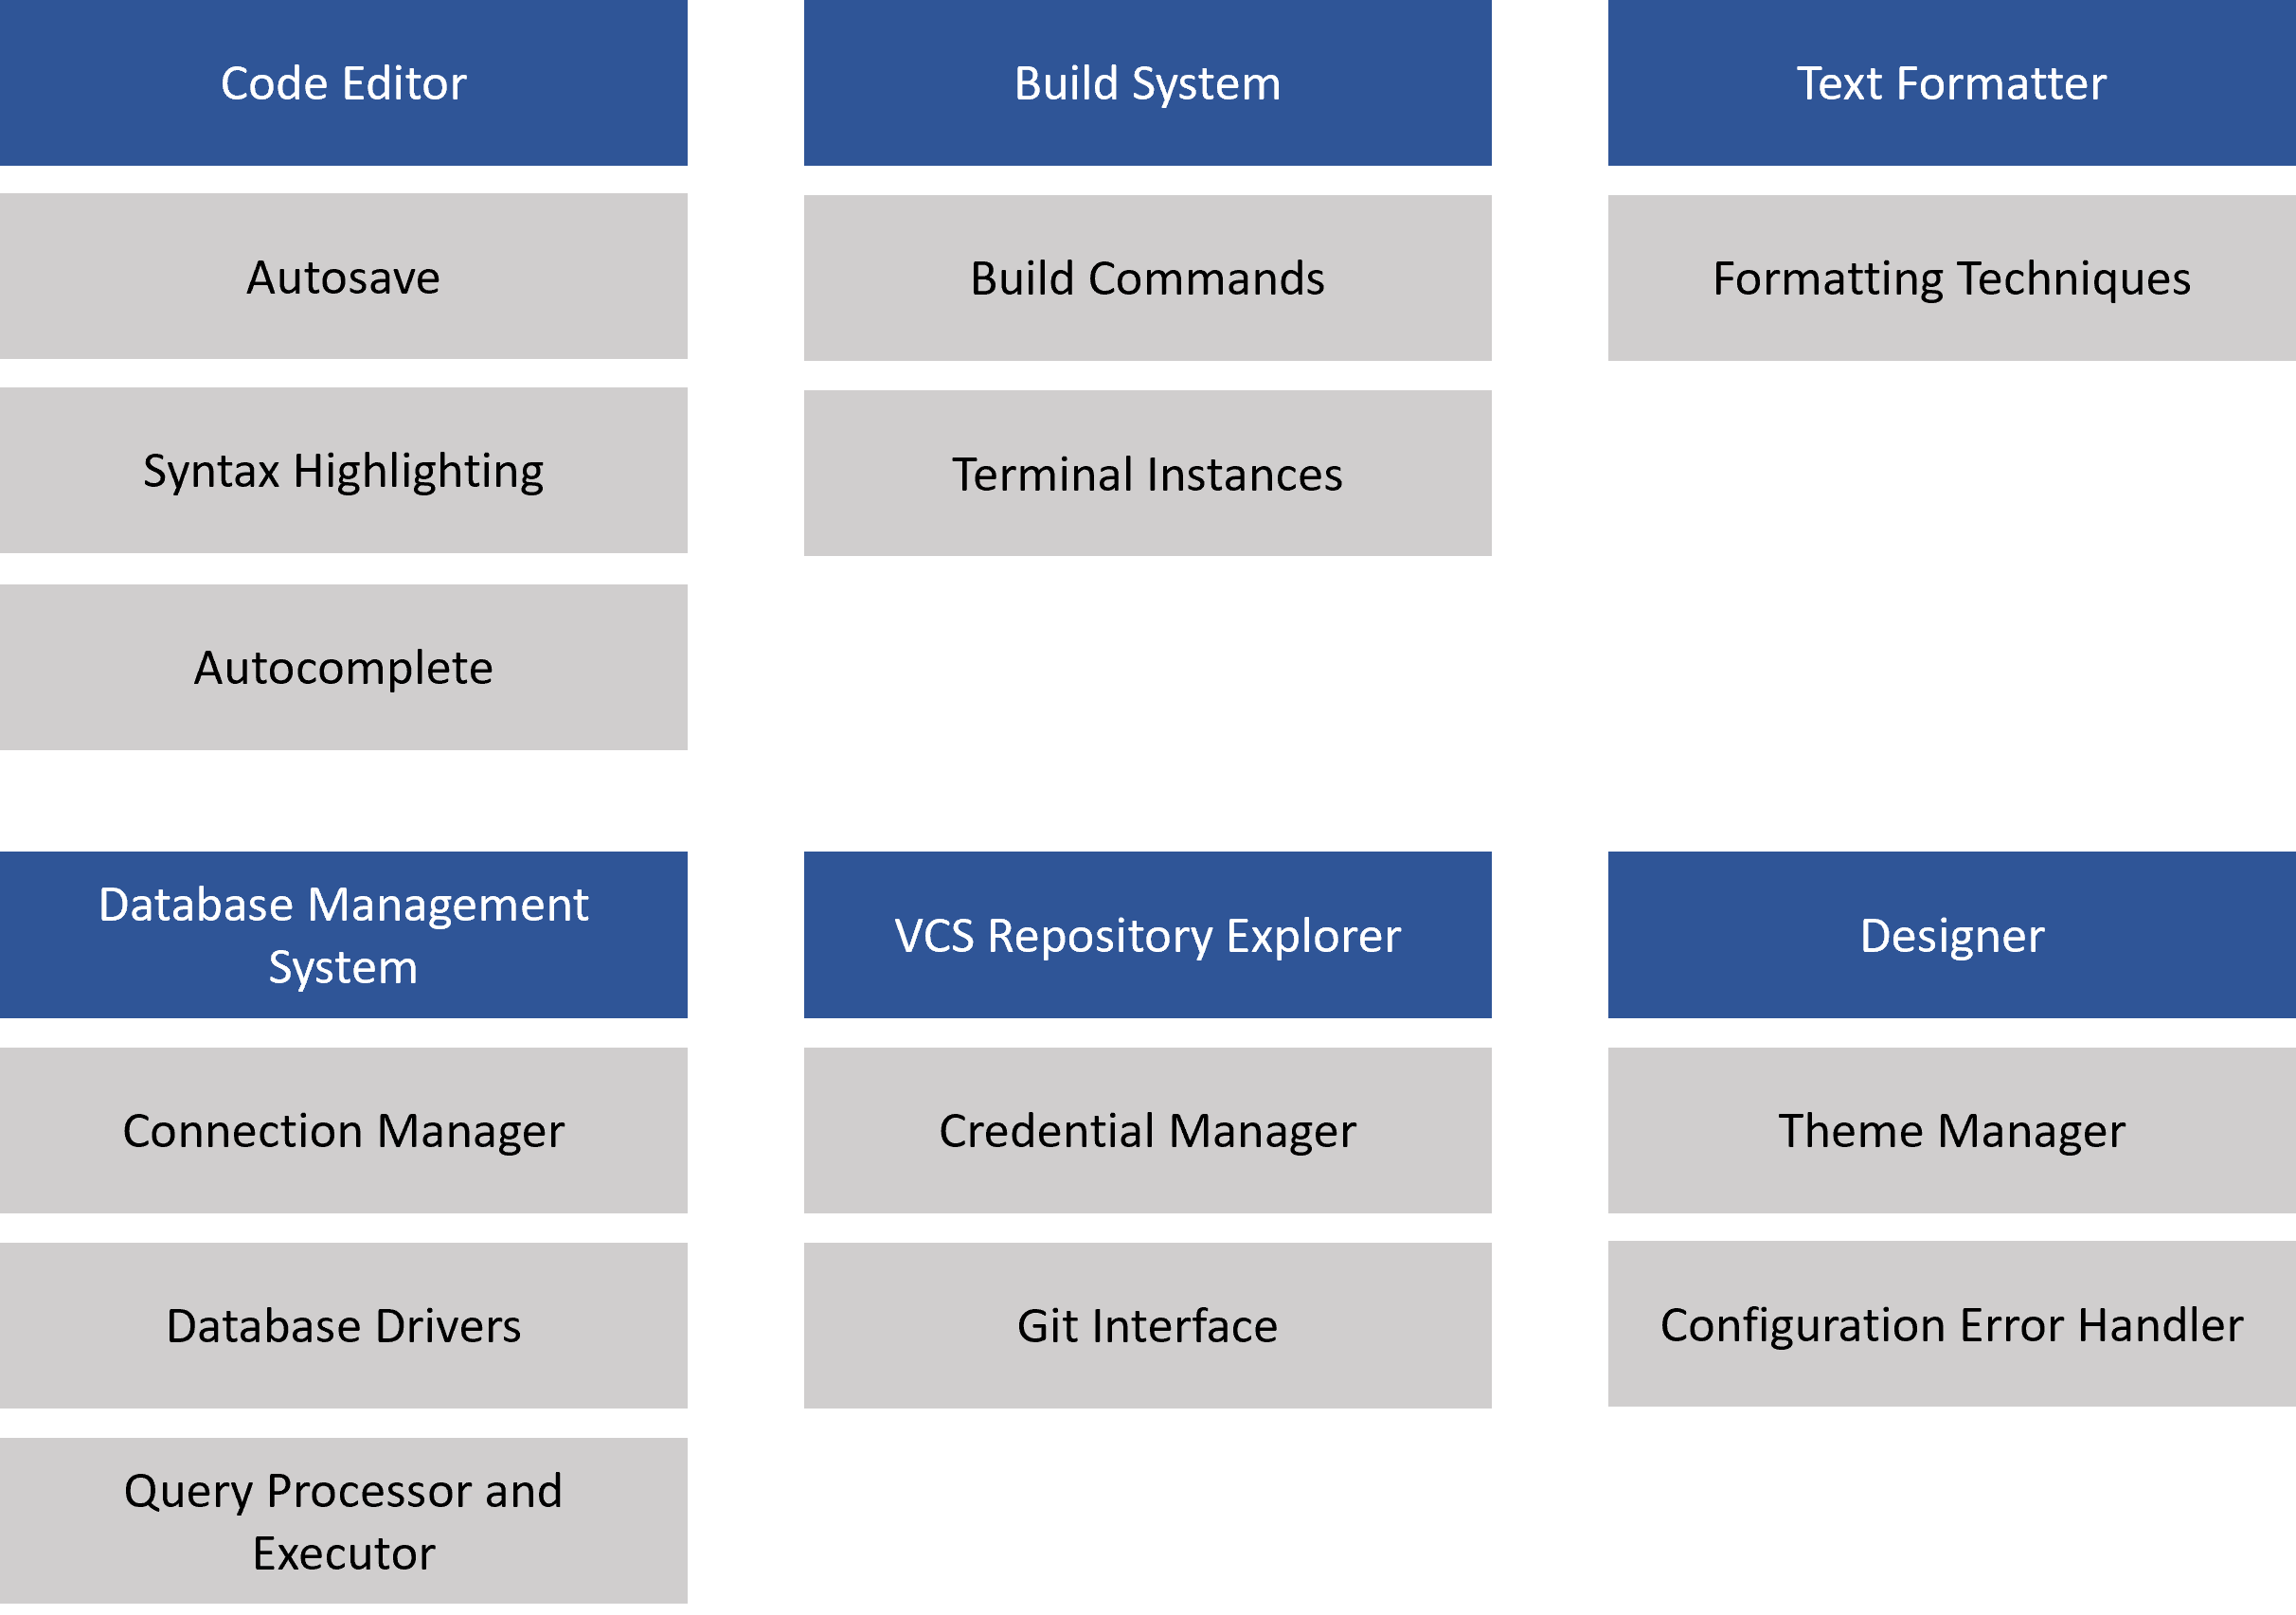
\includegraphics[width=0.6\textwidth]{images/structure.png}
\caption{The components that build up Pie}
\label{fig:fig2,1.}
\end{figure}

Code Editor provides the main capabilities of Pie. It handles the project's tab management, the instances of Scintilla, and it focuses on providing a friendly environment for the developer while writing code. The editor analyzes the extension of the opened file and initializes the syntax highlighting and autocomplete by sending a corresponding set of keywords and symbols to the Scintilla control. The component also renders HTML and Markdown files and provides proper handling of errors, when such a process fails. Going back to the independence of Pie's modules, the Code Editor works together with the Designer (component 6), when instantiating Scintilla controls, in order to provide syntax highlighting colors of the currently active theme.

The Build System allows users to add their own build commands and access them from the docked toolbar. It also handles the ConEmu terminal instances and launches every custom (or pre-defined) build command in a new terminal. Terminal tabs can also be created manually, whenever users need to input additional commands.

Text formatting capabilities were necessary, as people commonly do text-based convertions such as CSV (comma-separated values) to newline, or even backwards. Notepad++ is currently the best option for advanced text manipulation, and is often used as an extra tool during the development process, as IDEs do not provide formatting features. Pie's Text Formatter has been built for this purpose.  The tool supports common text formatting capabilities, accessible from an entire list of such actions. The list can be ordered alphabetically by the name of the formatting technique, its category or description. Users can also search through the existent actions by using the incorporated text box that updates the list in real time.

The Database Management System handles the persistence layer of Pie. It initializes a specific database connection drivers, based on several connection parameters. The connection parameters are stored in a configuration file which is read (and updated) by the manager whenever needed. This component also provides the "Run query against ..." button when a user right clicks the Scintilla control on an opened SQL file. Querying a table will result in Pie displaying a window with the output of the statement.

VCS Repository Explorer allows users to manage their local Git repositories by inspecting file statuses, viewing commit logs and pushing to/pulling from remote repositories. These actions are performed through a clean, user-friendly interface that gets opened in a new tab, whenever developers manually toggle it under the "Interface" menu element.

The Designer has influence over all of Pie's visual elements. It handles theme configuration files that can be manually added/removed by the users. The color schemes specified in the JSON-formatted data can control every aspect of the application: from the color of the windows, to the syntax highlighting color of a bracket in Scintilla. The users can also choose the theme's type: light or dark. This influences the colors of the icons (and arrows) present in Pie's controls.

\section{Architecture}

\subsection{The Model-View-Controller ("MVC") pattern}

Model-View-Controller (or "MVC") is a "pattern in software design commonly used to implement user interfaces, data, and controlling logic" \cite{mozilla-mvc}. It focuses on separating business logic from user interface code, in order to keep a cleaner project and increase its maintainability.

The MVC pattern relies on three components:

\begin{enumerate}
  \item model: defines data structures and business logic;
  \item view: defines the user interface of the application;
  \item controller: handles events, inputs and refreshes the view when needed. 
\end{enumerate}

Although this solution is a great way to separate concerns in all types of software products, including web applications where it is mostly used, Windows Forms doesn't directly implement this pattern and requires additional effort and code from the developer. I have decided not to implement it for one major reason: my code mostly relies on user interface processing. Moving logic from one place to another would result in several classes being defined only because the pattern dictates so. Entities (or models) are already defined as separate classes in Pie, so we can agree that, to a certain extent, I have integrated some aspects of the MVC pattern. However, these entities mostly resemble configuration data that is read from files or processed during the application's lifecycle.

Another advantage brought by the MVC pattern is on code testability \cite{mvc-testability}. In Pie's case, testing of business logic isn't favored because of its focus on handling user interface. It is true that several functionalities such as the Text Formatter (discussed in the next subsections) are built as input-output based services, meaning they are easy to test. However, implementing MVC over the entire application just to test several small functionalities isn't feasible. Unit testing on Pie should be done mostly on the user interface, and Microsoft already has provided solutions such as the UI Automation Framework \cite{ui-automation-framework} to do it for us.

\subsection{The file structure of the solution}

The following section describes the file structure of Pie. The application consists of a large number of C\# classes, grouped based on their purpose in folders for better readability. Figure 4.2 displays the structure of the project.

The "Forms" group consists of the windows visible to the user when interacting with the application. WinForms creates a C\# class for each Form added to the project.

"Services" typically have to do with logic that doesn't necessarily imply user interface processing. Most of the services interact with files, by performing reads and writes on them. This is how configuration data in Pie is persisted. Configuration data includes, but is not limited to, color schema definitions, database connections, and flags such as autosave and word wrap. There are several services that do more than file manipulation, such as "GitService" that calls the LibGit2Sharp API, besides handling credentials stored in .json files.

The folder named "Classes" contains the entities, commonly referred to as "models" in the MVC language. Services usually handle globally defined entities during the application runtime. For example, at the application start, the "BuildCommandService" reads all of the saved build commands from the config/build.json file and stores them in a list of "BuildCommand" objects, that is made visible when the user tries to launch a build command from the top menu strip.

"Enums" is used as a way to define types of elements. "DatabaseType" is used to convert user input (when creating a new database connection) to one of the three database management systems (MySQL, MSSQL or PostgreSQL). "TabType" has to do with the tab management system provided by the Code Editor component. A tab can be of four types: CODE, RENDER\_HTML, RENDER\_MD or GIT. This simply means that several interface elements of Pie do not open in a new window (such as the list of build commands or database connections), but they open as a new tab directly in the editor. I have implemented this, because it is more practical to switch between the tab containing the output of an HTML file and its source code, than to press a button to open a pop-up window with the output and later close it to continue with the implementation.

The "Resources" folder doesn't contain any source files or classes, but keeps icons and images used in Pie's controls. 

\begin{figure}
\centering
\framebox[0.7\textwidth]{%
\begin{minipage}{0.7\textwidth}
\dirtree{% This % is required
.1 pie. 
.2 Forms.
.3 Build Commands.
.4 AddBuildCommandForm.cs.
.4 BuildCommandsForm.cs.
.3 Databases.
.4 AddDatabaseForm.cs.
.4 DatabaseOutputForm.cs.
.4 DatabaseForm.cs.
.3 Format.
.4 FormatForm.cs.
.3 ....
.2 Services.
.3 BuildCommandService.cs.
.3 DatabaseService.cs.
.3 GitService.cs.
.3 ....
.2 Classes.
.3 GitCredentials.cs.
.3 FormatOption.cs.
.3 DatabaseConnection.cs.
.3 ....
.2 Enums.
.3 DatabaseType.cs.
.3 TabType.cs.
.3 ....
.2 Resources.
}
\end{minipage}
}
\caption{Pie's file structure, containing folders (Forms, Services, Classes, Enums, Resources) and C\# sources (*.cs)}
\end{figure}

\subsection{Event handlers in Form classes}

Pie's code mostly relies on event handling logic. Controls can also be inserted dynamically during the program's flow, besides dragging and dropping them from the toolbox. Based on events such as key presses or mouse clicks, controls are inserted, removed, shown, hidden or repositioned at runtime.
\chapter{Implementation}
\thispagestyle{pagestyle}

The following section will present the implementation of Pie's most important aspects, including handling of configuration files, applying color palettes to WinForms controls, tab management for the code editor and terminal instances, syntax highlighting for various languages, directory navigation logic, Find\&Replace logic with ScintillaNET's API, database connection handling, using LibGit2Sharp to manage repositories and text formatting algorithms. It will also display code snippets, along with screenshots of the application and paragraphs with additional explanation.

\section{JSON-based configuration in Pie}
\chapter{Usage Scenarios}
\thispagestyle{pagestyle}

In this chapter, I will present several usage scenarios for Pie, managing to detail how Pie can replace a code editor for daily activities. Every use case will be backed up by screenshots and paragraphs emphasizing on the application's interface.

\section{Writing HTML code and rendering it}

Code editing is the most common functionality accessed in Pie. The Scintilla editor is visible since the first start of the application, and code support will be made available after the user saves the content of the editor.

\begin{figure}[H]
\centering
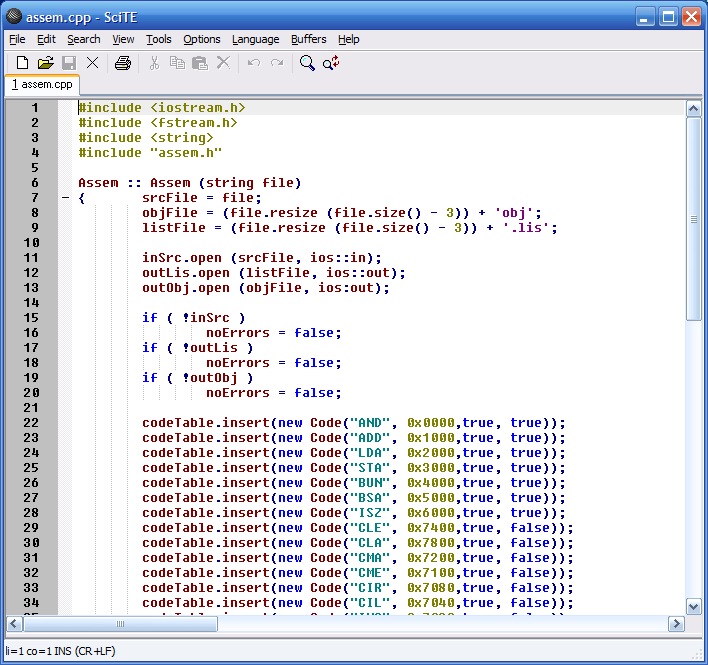
\includegraphics[width=0.7\textwidth]{images/scite.png}
\caption{Scintilla's syntax highlighting capabilities in the SciTE editor}
\label{fig:fig2,1.}
\end{figure}
\chapter{Conclusions}
\thispagestyle{pagestyle}

In this work, I have presented a method to enhance productivity in the software development field by introducing an application suitable for small-scale projects. In "State of the Art", I explored the history of code editors, from the punch card era to the present day. I also performed a comparison between my solution, Pie, and the most popular integrated development environments on the market. This comparison demonstrates that Pie not only includes all the essential features of an IDE but also offers an intuitive user interface that simplifies access to these features.

In the next chapter, "Technologies", I discussed the technologies that form Pie's building blocks, with a particular focus on Microsoft's Windows Forms, a mature user interface solution for the .NET framework. The "Application Structure" chapter introduced Pie's "components" and showcased several features of the editor, accompanied by screenshots.

A way of implementing the application's features using the C\# language was discussed in the "Implementation" chapter, where I also included code snippets explained in comments and additional paragraphs. Finally, the "Usage Scenarios" chapter illustrated the intended use cases for Pie.

Pie has been well received by the developer community, and an article about it is set to be published at the SACI (IEEE 18th International Symposium on Applied Computational Intelligence) 2024 conference in Timișoara. By staying in close contact with developers from Romania through various programming communities and forums, I have received valuable feedback that helped me take important decisions regarding future integrations for my product.

As future work, I plan on launching the application in a beta version in order to gather more feedback from its users. I consider that the best feedback is the one received by users actually testing the solution, not just reading about it. Gathering feedback will allow me to refine Pie's present features and also add additional ones, if needed.

I also plan to improve Pie's Git interface, as it does not provide all the features found in standalone repository explorers. Pie should also provide users the option to roll back changes in a file, inspect every change through the Git log, and perform branch operations like merge or rebase. The database manager is also set for an update, as it will support more relational database types and have better error handling.


% Look for building the .bib file on Overleaf documentation
\printbibliography
\thispagestyle{pagestyle}

\end{document}